Sparse coding inspired many early works in deep feature learning
\cite{SC,SAE,SAE2}, as well as early works in unsupervised learning of
convolutional feature hierarchies \cite{ConvSC}. All of these works rely
heavily on solving the sparse inference problem described in Chapter
\ref{chapter:related_work}.  However traditional iterative solvers can be
computationally expensive and are not formulated as functional mappings that
are amenable to network implementations \cite{FISTA}. The work by Gregor and
LeCun dubbed ``LISTA'' \cite{LISTA} proposed a specialized network architecture
for learning to predict sparse codes. However that work LISTA networks were
trained to directly predict the codes found using intirative inference
algorithms.  In this chapter we will empirically evaluate LISTA encoders under
a wider variety of conditions. This will include training convolutional LISTA
networks to learn sparse inference in convolutional dictionaries by directly
minimizing the lasso loss.

\section{Convolutional-LISTA} 

\begin{figure}
\centering
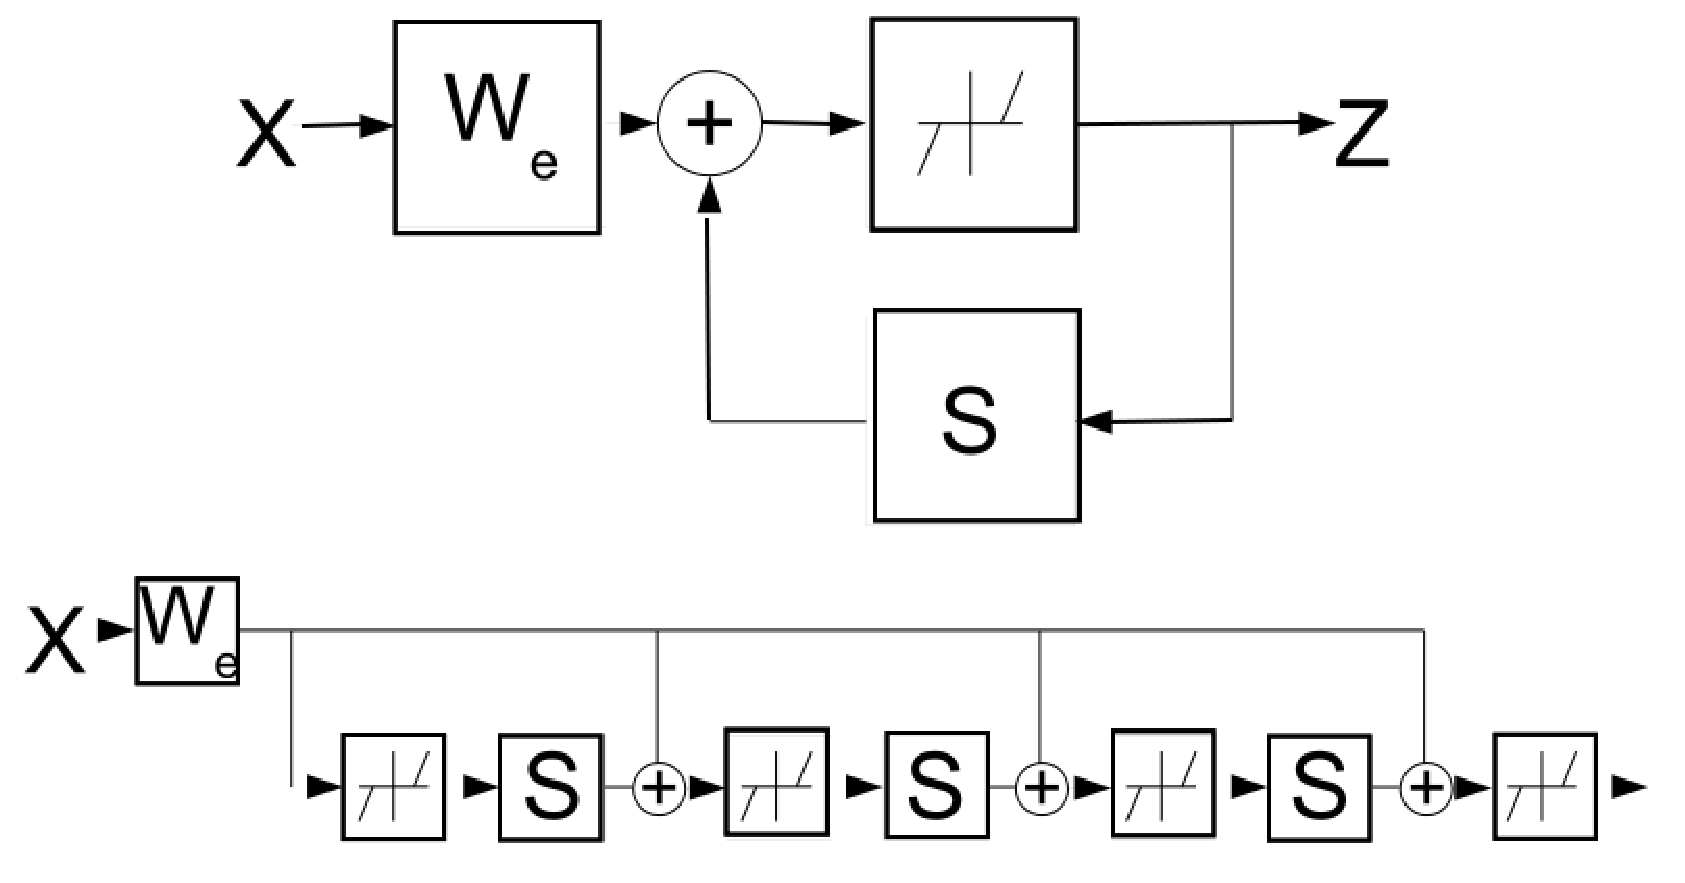
\includegraphics[scale=0.3]{./figures/LISTA/LISTA.pdf}
\caption{LISTA network architecture} 
\label{fig:LISTA} 
\end{figure}  

Recall the iterative ISTA algorithm for solving the relaxed sparse inference problem
known as the lasso was discussed in Chapter \ref{chapter:introduction}. 
Recall that the lasso loss is given by:
  
\begin{equation}
L_{lasso} = \frac{1}{2}\|X-W_dZ\| + \alpha |Z|_1 
\label{eqn:lasso} 
\end{equation} 

The LISTA network architecture is \emph{derived} by expressing the ISTA
algorithm as a recurrent network, and ``unrolling'' into a finite number of
loops with shared-weight stages.  The recurrent and unrolled networks
(three-loops) are shown in Figure \ref{fig:LISTA}. Note that
$S=I-\frac{1}{L}W_d^T W_d$, where $W_d$ is the decoder and $L$ is the upper
bound of $W_d^t W_d$.  The above network can be made convolutional by replacing
the linear operators $W_e$ and $S$ with convolutional filter banks. In order to
be able to compute the reconstruction error in Equation \ref{eqn:lasso}, the
convolutional synthesis operator must produce outputs of the same size as the
input. This can be accomplished by using ``same'' convolutions or by cropping
the input and computing the reconstruction error in the ``valid'' regions. As
in ordinary convolutional networks, each convolutional layer produces multiple
output planes. For example, if the encoder takes in images of 3-input planes
and produces $n$-output planes then the $S$ convolution stage takes in
$n$-input planes and produces $n$-output planes. Convolutional dictonaries are
massively overcomplete, making sparse inference a potentially much
harder problem \cite{ConvSC}. 
     
\begin{figure}
\centering
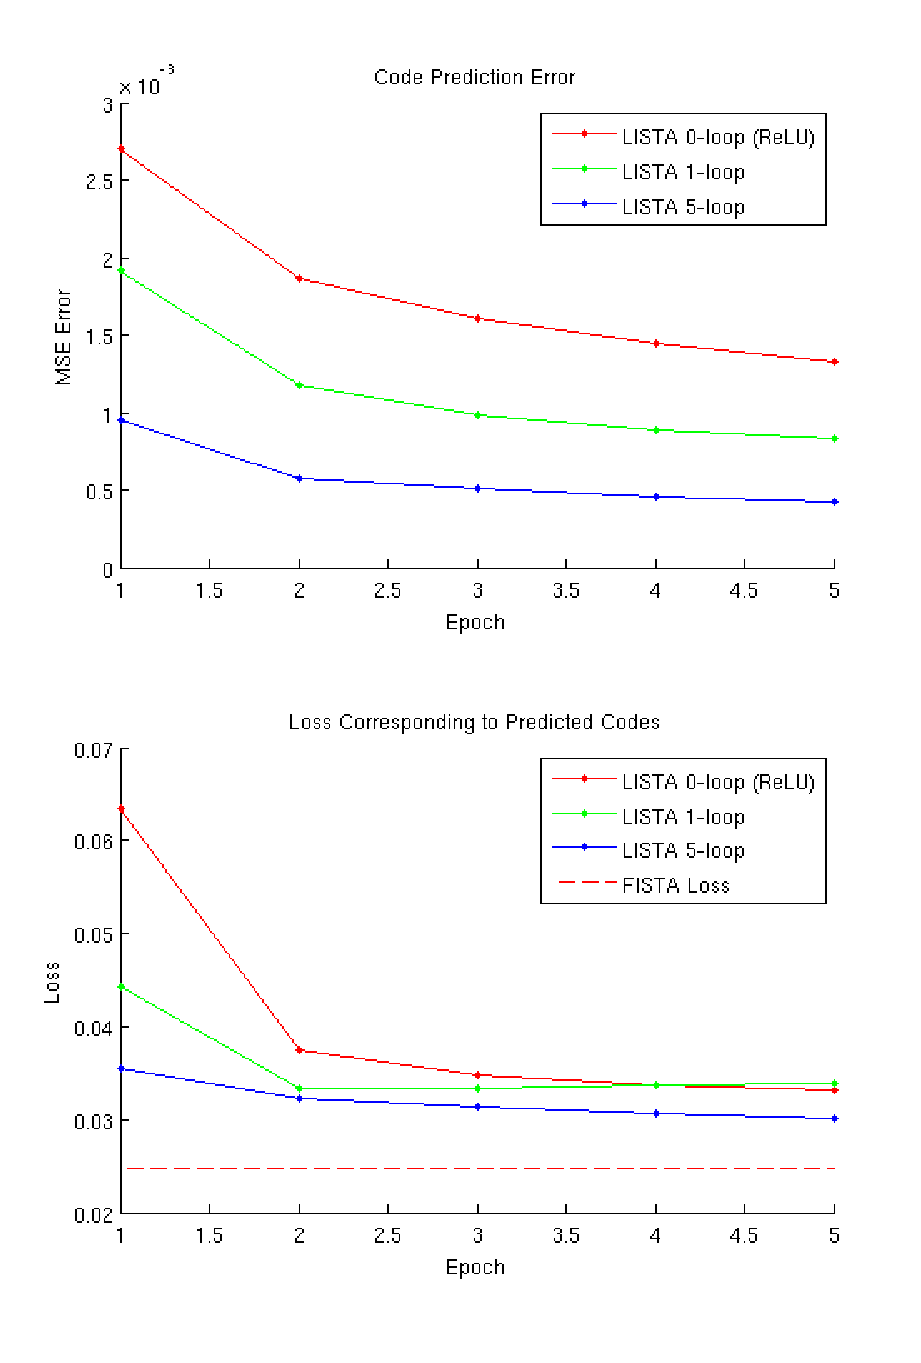
\includegraphics[scale=0.6]{./figures/LISTA/code_pred.pdf}
\caption{Sparse inference learning curves} 
\label{fig:LISTA} 
\end{figure}  


